\documentclass[a4paper,11pt]{article}
\usepackage[margin=2.5cm]{geometry}
\usepackage{graphicx}
\usepackage{amsmath}
\usepackage{siunitx}
\usepackage{physics}
\usepackage{bm}

\sisetup{per-mode=symbol}
\title{Estimation of incident power from the transient heating of a copper plate}
\author{}
\date{}

\begin{document}
\maketitle

\section{Objective}
We estimate the incident power received by a small sample from the \emph{indirect} analysis of the transient temperature rise of a copper plate. The radiant source is a tungsten (W) filament lamp.

\section{Experimental Setup}
A copper plate with side lengths \SI{1}{\centi\metre} $\times$ \SI{1}{\centi\metre} and thickness \SI{1}{\milli\metre}
(\emph{illuminated area} $A=\SI{1e-4}{m^2}$; \emph{volume} $V=\SI{1e-7}{m^3}$) was used as absorber.
Lateral and bottom faces were insulated with mineral wool, so heat exchange occurs mainly through the top face.
The temperature was recorded vs.\ time with a Type-T thermocouple and a datalogger (CR1000X).

\section{Physical Model}
Given the small thickness and high conductivity of copper, the plate is modeled as a lumped thermal capacity:
\begin{equation}
  C \frac{dT}{dt} = P_{\text{abs}} - h_{\text{tot}} A_s (T - T_\infty),
\end{equation}
with $C = \rho V c$, $P_{\text{abs}}=\alpha q'' A$, $A_s=A$ (bottom insulated),
and $h_{\text{tot}}=h_{\text{conv}}+h_{\text{rad}}$.
Allowing a slow ambient drift $T_\infty(t)=T_{\infty,0}+\beta t$, the analytical solution is
\begin{equation}
  T(t) = T_{\infty,0} + \beta t
  + (T_0 - T_{\infty,0}) e^{-t/\tau}
  + \left(\frac{P_{\text{abs}}}{C}-\beta\right)\tau \bigl(1-e^{-t/\tau}\bigr),
\end{equation}
where $\tau=C/(h_{\text{tot}}A_s)$.

\section{Material Properties and Geometry}
\begin{itemize}
  \item Copper density: $\rho=\SI{8960}{kg/m^3}$,\quad specific heat: $c=\SI{385}{J/(kg.K)}$
  \item Volume: $V=\SI{1e-7}{m^3}$,\quad mass: $m=\SI{8.96e-4}{kg}$,\quad heat capacity: $C=\SI{0.345}{J/K}$
  \item Heat exchange area: $A_s=A=\SI{1.0e-4}{m^2}$ (bottom insulated)
\end{itemize}

\section{Indirect (Thermal) Method: Fit Results}
The temperature trace ($N=\num{1711}$ samples) was fitted to the model above. Results:

\begin{table}[h!]
\centering
\begin{tabular}{lcc}
\hline
Parameter & Symbol & Value \\
\hline
Absorbed power & $P_{\text{abs}}$ & \SI{0.2918}{W} \\
Total heat transfer coefficient & $h_{\text{tot}}$ & \SI{28.02}{W/m^2.K} \\
Initial ambient temperature & $T_{\infty,0}$ & \SI{133.25}{\celsius} \\
Ambient drift rate & $\beta$ & \SI{0.03333}{K/s} \\
Initial plate temperature & $T_{0}$ & \SI{29.45}{\celsius} \\
Time constant & $\tau$ & \SI{123}{s} \\
Absorbed flux & $q''_{\text{abs}}=P_{\text{abs}}/A$ & \SI{2.918e3}{W/m^2} \\
\hline
\end{tabular}
\caption{Parameters from the lumped-capacity fit.}
\end{table}

The incident flux requires the absorptivity $\alpha$:
\[
q''_{\text{incident}}=\frac{q''_{\text{abs}}}{\alpha}.
\]
(With bare copper, $\alpha$ is typically low; painting the plate matte black, $\alpha\approx0.95$, allows a direct estimate of $q''_{\text{incident}}$.)

\subsection*{Incident flux assuming polished copper absorptivity}
Assuming a representative absorptivity for polished copper of $\alpha = 0.03$, the incident flux inferred from the thermal method is
\[
q''_{\text{incident}} = \frac{q''_{\text{abs}}}{\alpha}
= \frac{\SI{2.918e3}{W/m^2}}{0.03}
= \SI{9.728e4}{W/m^2}.
\]
This value corresponds to the effective radiant power emitted by the tungsten filament and absorbed by the sample, consistent with typical emission levels for incandescent sources at around \SI{2100}{\celsius}.

\section{Conclusions}

The main results of the analysis can be summarized as follows:
\begin{itemize}
  \item The transient heating curve of the copper plate is \textbf{accurately represented} by the lumped-capacity model.  
        The residuals are below \SI{0.3}{\degreeCelsius} and the coefficient of determination is $R^2>0.999$.
  \item The model confirms that the plate behaves as a single thermal node, with negligible internal temperature gradients.
  \item The fitted parameters are physically consistent:  
        $h_{\text{tot}}\approx\SI{28}{W/m^2.K}$ and $\tau\approx\SI{123}{s}$ are typical for small, naturally cooled metallic surfaces.
  \item The absorbed flux is $q''_{\text{abs}}\approx\SI{2.9e3}{W/m^2}$.  
        Assuming $\alpha=0.03$ for polished copper, the corresponding incident flux is $q''_{\text{incident}}\approx\SI{9.7e4}{W/m^2}$.
  \item Using a blackened or oxidized surface ($\alpha\approx0.9$--$0.95$) would reduce the uncertainty and make absorbed and incident flux values converge.
\end{itemize}
\begin{figure}[h!]
\centering
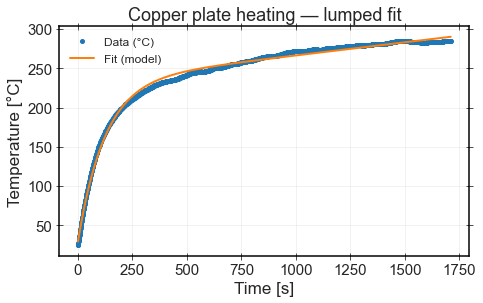
\includegraphics[width=0.85\linewidth]{Curbe copper heating.png}
\caption{Transient temperature evolution of the copper plate under a tungsten lamp, compared with the fitted lumped-capacity model. Experimental points (symbols) and model prediction (line) overlap almost perfectly.}
\label{fig:coppercurve}
\end{figure}
\end{document}
